\section{Teórico 1/2}

  \definicion{Topic:} Forces, stresses, geometry optimisation.

  \definicion{Speaker:}	Pietro DELUGAS (SISSA, Italy).

\subsection{Parámetros estructurales}

  Un sistema queda definido a partir del número y tipo de iones, donde el tipo queda descripto a partir del PP, junto a las posiciones que ocupa cada uno, determinando la estructura.

  La estructura de un sistema periódico queda descripta por:
    \begin{itemize}
      \item Los parámetros de red: $\vec{a}_1$, $\vec{a}_2$ y $\vec{a}_3$.
      \item Las posiciones atómicas: $\vec{r}_I$
    \end{itemize}

  Como la modificación de los parámetros de red alteran las posiciones atómicas, se utilizan coordenadas cristalinas fraccionarias, donde la posición atómica queda expresada a partir de los parámetros de red.
    $$\vec{r}_I = \sum_{i=1}^3 x_i \vec{a}_i \quad ; \quad 0 \leq x_i \leq 1$$

  La energía potencial $E(\vec{r}_I, \vec{a}_i)$ termina siendo la PES (Potential Energy Surface) del sistema bajo la aproximación de Born-Oppenheimer: esta es la función a minimizar.

\subsection{Fuerzas}

  La PES debe ser derivable ya que la fuerza es el opuesto de la derivada de las interacciones interelectrónicas e internucleares respecto a las posiciones.
    $$F_I = - F_I^{el} - \frac{e^2}{2} \frac{\partial}{\partial \vec{r}_I} \sum_{I\neq J} \frac{Z_I Z_J}{\norm{\vec{r_I} - \vec{r_J}}}$$

  El teorema de Hellmann-Feynman puede ser aplicado en DFT. El mismo establece que la derivada de la energía total $E$ respecto a un parámetro continuo $\lambda$ es igual al valor de expectación de la derivada del Hamiltoniano respecto a dicho parámtro. Así, una vez que la distribución espacial de los electrones ha sido determinada al resolver la ecuación de Schrödinger, todas las fuerzas del sistema puede usarse recurriendo a la electrostática clásica.
    $$\frac{d E}{d \lambda} = \expval{\sfrac{d H}{d \lambda}}{\Psi}$$

  De este modo, la contribución electrónica $F_I^{el}$ puede determinarse como el valor de expectación de las derivadas del potencial externo aplicado.
    $$F_I^{el} = - \frac{\partial E}{\partial \vec{r}_I} = - \sum_v f_v \expval{\sfrac{\partial V}{\partial \vec{r}_I}}{\psi_v} = - \int n(\vec{r}) \frac{\partial V}{\partial \vec{r}_I} d \vec{r}$$

  La idea de calcular las fuerzas como un valor de expectación es válida sólo si estamos realmente en convergencia: la precisión de las fuerzas dependerá de que estemos cerca de la autoconsistencia. Esto se debe a que en realidad tenemos un segundo término al derivar la energía, el cual se anula cuando estamos en un mínimo:
    $$\frac{\partial E}{\partial \vec{r}_I} = \int n(\vec{r}) \frac{\partial V}{\partial \vec{r}_I} d \vec{r} + \int \frac{\delta E}{\delta n(\vec{r})} \frac{\partial n (\vec{r})}{\partial \vec{r}_I} d \vec{r}$$

  En QE, pw.x imprime un estimado de este segundo término al final de la autoconsistencia que puede servir como una correción aproximada. Durante una relajación o una dinámica debemos monitorear estos valores: deben ser algún orden de magnitud menor que las fuerzas calculadas. De lo contrario el programa emite una advertencia.

\subsection{Tensión y estrés}

  Dijimos que cambiar los valores de los parámetros de red implica una deformación uniforme del sistema. Esta queda descripta por el tensor de tensión $e_{\alpha \beta}$. La transformación es lineal
    $$\vec{r}_{\alpha}^{'} = \sum_{\beta} (\delta_{\alpha \beta} + e_{\alpha \beta}) \vec{r}_{\beta}$$

  El tensor de estrés es la derivada de la energía por unidad de volumen con respecto a la tensión.
    $$\sigma_{\alpha \beta} = -\frac{1}{\Omega} \frac{\partial E}{\partial e_{\alpha \beta}}$$

  Sólo la contribución simétrica del tensor $e_{\alpha \beta}$ da lugar a una deformación efectiva, afectando la energía, ya que la contribución antisimétrica es simplemente una rotación.

  La traza del tensor de estrés está relacionada a la presión según
    $$P = \frac{1}{3} \sum_{\alpha} \sigma_{\alpha \alpha} $$

  mientras que las componentes no diagonales son el estrés de corte (deformaciones no paraleas a los planos de la celda unidad).

  Como el estrés es una primera derivada de un parámetro externo, el teorema de Hellmann-Feynman puede aplicarse. En este caso no depende explícitamente de las posiciones iónicas, sino que es la derivada de la energía cinética, la de Hartree y la de XC con respecto a una deformación uniforme. Esto lleva a que involucra las componentes de las funciones de onda, las cuales dependen a su vez de la base de PWs usada.

\subsubsection{Smooth cutoff}

  Evaluar la energía y el estrés puede dar discontinuidades si el cutoff no fue convergente, teniendo que usar valores más grandes. Una alternativa es usar smooth cutoff: creamos una región donde las PW entran y salen del conjunto base con regularidad, teniéndose en cuenta cuando se evalúa el estrés y la energía.

  Esto se logra modificando el funcional de energía cinética por lo que las PW de borde se vuelven caras.
    $$T (\vec{G}) = \underbrace{\norm{\vec{G}}^2}_{\text{original}} + \underbrace{Q_{cut} \left[ 1 + erf\left( \frac{\norm{\vec{G}}^2 - E_{cfix}}{\sigma} \right) \right]}_{\text{smooth}}$$

  Cuando $\vec{G}^2 - E_{cfix} < 0 \wedge \abs{\vec{G}^2 - E_{cfix}} \ll \sigma $ la función error tiende a $-1$, por lo que $T (\vec{G}) \rightarrow \norm{\vec{G}}^2$. A medida que $\vec{G}^2$, empieza a haber contribuciones no nulas. Sin embargo, la transición es suave y no brusca.

  En QE tengo las siguientes variables del input en pw.x (Fig. \ref{fig:smooth}):
    \begin{itemize}
      \item $ecfied \rightarrow$ energía por encima de la cual las PWs alcanzan el máximo costo.
      \item $qesigma \rightarrow$ ancho a partir del cual se empieza a sumar este costo extra.
      \item $qcutz \rightarrow$ valor del costo extra de energía.
    \end{itemize}

    \begin{figure}[H]
        \centering
        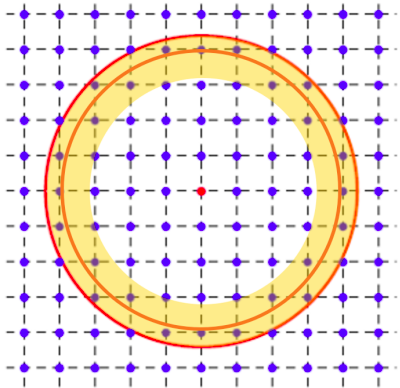
\includegraphics[scale = 0.6]{figs/D3/smooth.png}
        \caption{Cómo afectan las variables del smooth cutoff en la grilla sobre el $G$-espacio: $ecfied$ es el círculo naranja, $qesigma$ es el anillo amarillo t $ecutwfc$ es el círculo rojo.}
        \label{fig:smooth}
    \end{figure}

  Tenemos entonces que el smooth cutoff nos permite hacer una evaluación más regular del estrés y, además, no necesitamos aumentar $ecutwfc$.

\subsection{Métodos de optimización estructural}

  En pw.x se pueden hacer dos tipos de optimizaciones estructurales:
  \begin{enumerate}
    \item Manteniendo fijo el tamaño de celda: $calculation = 'relax'$. Se dan las posiciones atómicas y las mismas cambian según las fuerzas.
    \item Con tamaño de celda variable: $calculation = 'vc-relax'$. Se dan las posiciones atómicas y el tensor de tesión de la celda y las mismas cambian según las fuerzas y el tensor de estrés.
  \end{enumerate}

  Se tienen 2 algoritmos para para relajar:
    \begin{enumerate}
      \item \textbf{BFGS:} es un algoritmo cuasi-Newtoniano. Es el que se hace por defecto: $ion_dynamic='bfgs'$ y $cell_dynamics='bfgs'$
      \item \textbf{Quickmin:} es una dinámica de Verlet amortigüada. Debo decirle $ion_dynamic='damp'$ y $cell_dynamics='damp-pr'$ o $cell_dynamics='damp-w'$
    \end{enumerate}

\subsubsection{Quickmin}

  El mecanismo de amortiguación extrae energía cinética del sistema a medida que el sistema va cayendo al mínimo. Este algoritmo elimina cualquier componente de velocidad generalizada cuya dirección se oponga a la componente conjugada de la fuerza generalizada.

  Aunque el algoritmo es robusto ya que funciona incluso estando lejos del mínimo, requiere cierta experiencia con MD para establecer el time step. Suele ser más lento que BFGS: se suele usar primero un BFGS y luego el quickmin.

\subsubsection{BFGS}

  Es un algoritmo muy útil tanto para celda fija como para celda variable. En las proximidades de un punto de equilibrio $\vec{r}^{eq}$ ($\nabla E (\vec{r}^{eq}) \approx 0$) se asume una forma cuadrática para $E(\vec{r})$ tomando la Hessiana $\mathcal{H}$.
    $$E(\vec{r}) \approx E(\vec{r}^{eq}) + \frac{\vec{r} - \vec{r}^{eq}}{2} \mathcal{H} (\vec{r} - \vec{r}^{eq})$$

  Dados dos puntos $\vec{r}_1$ y $\vec{r}_2$ y sus respectivos gradientes $\vec{g}_1$ y $\vec{g}_2$, se tiene queda $\vec{g}_2 - \vec{g}_1 = \mathcal{H} (\vec{r}_2 - \vec{r}_1)$. Luego $\vec{g}_2=0$ si $\vec{r}_2 = \vec{r}_1 - \mathcal{H}^{-1} \vec{g}_1$ (Paso de Newton-Taphson).

  En la práctica se tiene una secuencai de cálculos en las posiciones $\vec{r}_i$.
    $$\vec{r}_{i+1} = \vec{r}_i + T_k^L \frac{\vec{s}_k^{NR}}{\norm{\vec{s}_k^{NR}}} \quad ; \quad \vec{s}_k^{NR} = - \mathcal{H}_k^{-1} \vec{g}_k$$

  donde $T_k^L$ se conoce como radio de confianza el cual determina cuánto nos vemos en la dirección dictada por $\vec{s}_k^{NR}$.

  Para el paso siguiente debemos actualizar la Hessiana de una manera particular la cual involucra diferencias entre gradientes.

  En cada uno de los pasos también se actualiza $T_k^L$ de manera tal que satisfaga las dos condiciones de Wolfe:
    \begin{enumerate}
      \item \textbf{Decrecimiento suficiente:} la nueva energía debe ser menor que cierto valor, sino $T_k^L$ debe acortarse.
        $$E_{new} \leq E_{old} + \omega_1 T_k^L \vec{g}\cdot \vec{s}_k$$
      \item \textbf{Curvatura:} si la nueva pendiente es muy alta, el $T_k^L$ es aumentado.
        $$\vec{g}_{new} \cdot \vec{s}_k \geq \omega_2 \vec{g}_{old} \cdot \vec{s}_k$$
    \end{enumerate}

  Los valores $\omega_{1}$ y $\omega_{2}$ se pueden fijar en el input. De lo contrario, el programa usa los valores por default.

\subsubsection{Características de la optimización estructural}

  \begin{itemize}
    \item Permite encontrar únicamente el mínimo más cercano, ya que no tiene la posibilidad de sortear barreras de activación.
    \item En principio no rompe la simetría del cristal, salvo errores por ruido numérico. Esto permite encontrar mínimos atados a la simetría dada puesto que puede haber diferentes mínimos asociadas a distintas simetrías.
    \item Durante una vc-relax el conjunto de PWs se mantiene constante a pesar de que los parámetros de red van cambiando. Esto hace que el resultado final no sea exactamente igual a lo que uno obtendría al comenzar la corrida de cero con el mismo cutoff ya que ambas bases no son iguales. Una vez obtenidos los vectores de red optimizados, el programa recalcula la energía con la base asociada a estos nuevos valores.
    \item Utiliza tanto las energías como las fuerzas para ubicar el mínimo. Si la SCF no fue convergente, el algoritmo no será convergente o dará lugar a errores. El error en las fuerzas es lineal, mientras que el error en las energías es cuadrático.
  \end{itemize}

\subsection{Born-Oppenheimer MD}

  Asumiendo un comportamiento clásico para los núcleos y los electrones en el estado fundamental, recurrimos a un Lagrangiano para describir el movimiento nuclear. Las ecuaciones de movimiento son entonces las ecuaciones de Newton usuales, las cuales pueden discretizarse e integrarse. Esto es lo que se conoce como MD \emph{sobre la superficie BO} donde los electrones se encuentran siempre en su estado fundamental instantáneo.

  El cálculo puede hacerse recurriendo a diversos algoritmos como Verlet o velocity Verlet.

  Algunas cosas a tener en cuenta son:
    \begin{itemize}
      \item El time step debe ser tan grande como sea posible, pero lo suficientemente pequeño como para poder seguir el movimiento nuclear con precisión. Se tiene que
        $$\Delta t \approx 0.01 - 0.1 \Delta t_{max} \quad ; \quad \Delta t_{max} = \frac{1}{\omega_{max}}$$
      donde $\omega_{max}$ es la frecuencia del modo vibracional (fonón) más rápido que tengamos en el sistema.
      \item Las fuerzas deben ser los suficientemente precisas como para que la energía se conserve paso a paso. De lo contrario, se observa un drift energético.
      \item Una BOMD es computacionalmente cara (No me la counter strike). A veces conviene hacer CPMD.
    \end{itemize}

\section{Q\&A 1/2}

    \definicion{Why keep the previous grid during the optimization cycle? Since the meat of the process is: scf --> optimize --> scf --> ... --> convergence ; why does one not consider the new lattice vectors? Why not adjust the cutoff accordingly at every step as it is done in the very last step of the optimization (I think), why keep the ellipse instead of the circle for the entire optimization? Is it a convergence issue?}

    or computational efficiency. reallocating everything is expensive

    \definicion{Does the penalty for high G components you were mentioning (the one with the erf) alleviate these effects or is it unrelated? I have not understood where this applies. I have not used the related flags so far in my calculations, in what cases should I bother with these parameters?}

    yes in principle any G  in the buffer zone has negligible weight in the computation but any G in there enters smoothly in the computation if its lenght become shorter and the stress derivative of the kinetic energy functional takes into account the change in energy of the Gs in the buffer zone

    \definicion{If local minima are an issue can you give a bigger kick to the system in order for it not to get trapped there (something analogous to what happens in ML algorithm since you are in a very similar optimization problem optimized by gradient descent)? Does it make sense to start a calculation with a big kick, see where the problem starts oscillating and then reduce the kick around that point with another calculation (or even do this automatically) ?}

    yes with complicated landscapes there are many methods not implemented directly in QE but that use QE as a force engine

    \definicion{When I do the relax calculation, in the .out file there is the information about the forces. What kind of information does this total force and  DFT-D3 dispersion force give us?}

    the one is just the amount of Forces due to DFT-D3 that is a post-DFT correction to forces. If you see there is also the warning about the fact that the dft forces have a magnitude comparable with the force. They are both very small though you should be close to the minimum

    \definicion{In the relax calculation, what does the 'upscale' parameter do to the ions?}

    Nothing: it sets a maximum value for scf threshold tightening, avoiding to end up with too small scf thresholds and never get to convergence

    \definicion{In which cases I would choose Ion-dynamics instead bfgs?}

    In cases where bfgs doesn't converge it could be useful

    \definicion{there is any way to get a good trade-off between the energy convergence thresh. and the force conv thresh? A general rule}

    Usually its a good idea to stick to the defaults, if you need to relax the system more you can tighten the criteria in a follow up calculation

    \definicion{s there a way to estimate how much memory I will use for the process? My question is because I usually use a cluster and I need to give these information before run a code.}

    There is a memory estimate written in the output of QE

    \definicion{Thinking in the Gamma point trick here, to reduce the expensive cost of optimization, should we use the converged k points or could we assume in general using less points its not going to affect strongly the optimized coordinates. (then use more kpoints in next calculations)}

    Ideally, we use the converged k points. But, as we use a supercell we reduce the k-point accordingly.

    \definicion{why at this example in vc-relaxation, you use 6 6 4 k points, not symmetric?}

    As we use a hexagonal cell, a=b !=c, so having the same k points grid wont be accurate. The value of the k points should be inverse  proportional to the real space distance

    \definicion{Why does it use 'm-p' for Zn? If I do not know, would I do the study of convergence?}

    M-P is one of the best smearing schemes for metallic systems. It could gives very serious problems for insulators.

    \definicion{What is the definition of force convergence threshold? Does it mean that the force of each atom less than the threshold?}

    Yes. Default is 1e-3 Ry/Bohr.

\section{Teórico 2/2}

    \definicion{Topic:} Chasing saddle points: the NEB method.

    \definicion{Speaker:}	Anton KOKALJ (Jožef Stefan Institute, Slovenia).

\subsection{Procesos activados}

  Se conoce como proceso activado a cualquier proceso caracterizado por barreras de activación, las cuales quedan determinadas por los saddle. Dada una PES se tienen infinitos caminos de reacción que conectan el estado inicial con el final. Se conoce como MEP (Minimum Energy Path) al camino de reacción más probable a $0\ K$. Cuando recorremos el MEP, el saddle determina el estado de transición (Fig. \ref{fig:saddle}).

  \begin{figure}[H]
      \centering
      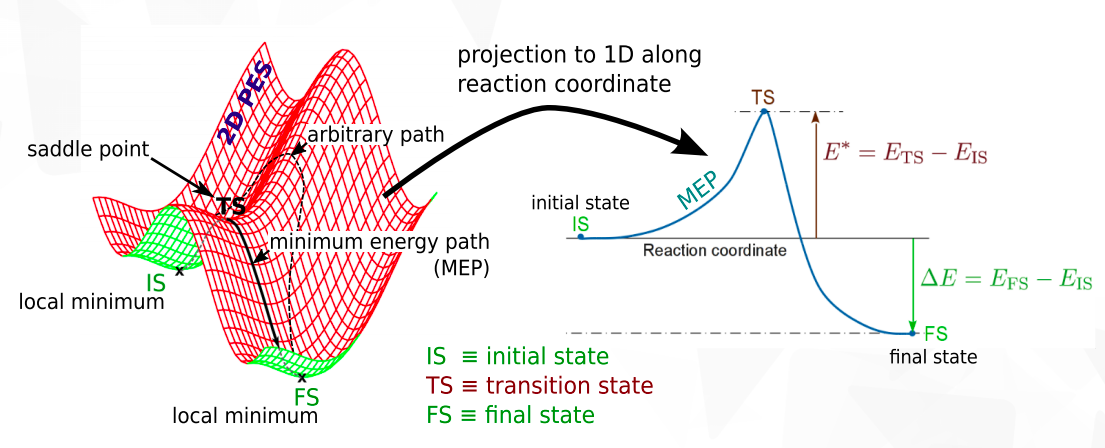
\includegraphics[scale = 0.4]{figs/D3/saddle.png}
      \caption{Proyección bidimensinal de una PES marcando sus puntos más importantes. Tomando el MEP se puede hacer una proyección unidimensional.}
      \label{fig:saddle}
  \end{figure}

  La importancia de la energía de activación radica en que es un muy buen criterio para decidir si cierto proceso activado es cinéticamente posible a cierta temperatura y, de serlo, qué tan rápido es. La constante de velocidad es
    $$k = \nu \exp(-E^{*} \beta) \quad ; \quad \nu = \frac{\prod_{j=1}^{3N} \nu_j^{IS} }{\prod_{j=1}^{3N-1} \nu_j^{TS}}$$

  Aunque típicamente $\nu \approx 10^{13} s^{-1}$, en realidad depende del tipo de proceso: para la desorción suele ser $\nu \approx 10^{16} s^{-1}$ por ejemplo (ver Surf. Sci. Rep. 12, 183-242 (1991)).

  En el contexto del análisis de procesos activados, se conoce como \emph{imagen} a una dada configuración del sistema completo. Vamos a usar además un vector $\vec{R}$ que representa en realidad al vector $3N$ dimensional con todas las coordenadas de los $N$ núcleos. Así $\vec{R}^{(n)}$ es el vector posición de los $N$ núcleos en la $n$-ésima iteración.

\subsection{NEB}

  El estado inicial y el final son mínimos, por lo que deben encontrase mediante métodos de optimización. Por otro lado, encontrar el saddle es bastante más complicado. Un método para encontrarle es el NEB (Nudged Elastic Band). La idea es la siguiente (Fig. \ref{fig:NEB}):
    \begin{enumerate}
      \item Conectamos el estado inicial y el final con una \emph{banda elástica}, la cual es tan elástica como sea necesario, \emph{i.e.} no se puede cortar nunca.
      \item Relajamos la bandita mediante fuerzas ortogonales ($\vec{F}_{\perp}$) a la misma.
      \item Eventualmente se alcanaz $\vec{F}_{\perp} = 0$. La bandita resultante marca el MEP y determina el saddle.
    \end{enumerate}

    \begin{figure}[H]
        \centering
        \subfigure[]{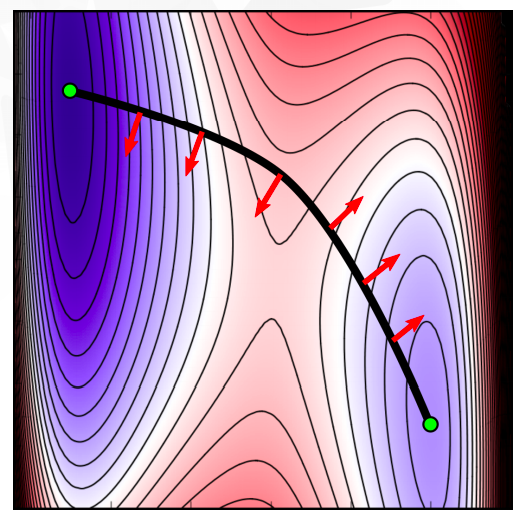
\includegraphics[scale = 0.30]{figs/D3/NEB_2a.png}}
        \subfigure[]{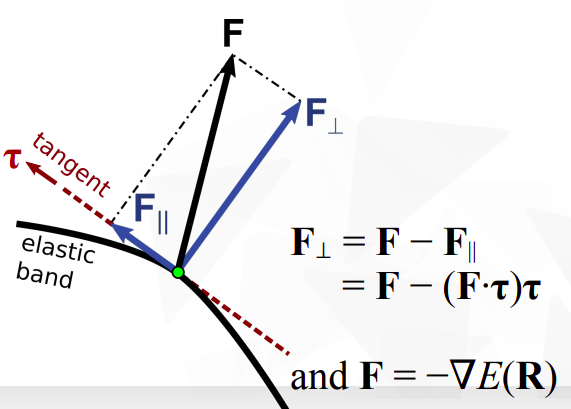
\includegraphics[scale = 0.25]{figs/D3/NEB_2b.png}}
        \subfigure[]{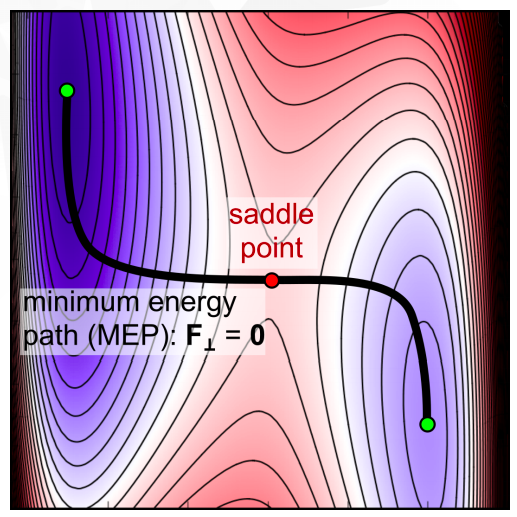
\includegraphics[scale = 0.30]{figs/D3/NEB_2c.png}}
        \caption{(a) Cómo conectamos el estado inicial con el final en NEB: la línea negra representa la banda elástica, mientras que las flechas rojas son las contribuciones ortogonales de la fuerza. (b) Descomposición de la fuerza aplicada sobre la bandita. (c) Resultado final donde $\vec{F}_{\perp} = 0$: la bandita marca el MEP.}
        \label{fig:NEB}
    \end{figure}

  Computacionalmente necesitamos discretizar la bandita elástica en una cantidad finita de imágenes: la fuerza perpendicular es calculada sobre estas imágenes. El problema de la discretización es que no preserva la distancia entre imágenes, lo cual puede dar lugar a distintos problemas a medida que avanzan las iteraciones. Para solucionar este problema, las imágenes son conectadas mediante resortes (Fig. \ref{fig:disc}), los cuales sólo actuan a lo largo del camino de reacción para mantener la distancia inter-imágenes.

  \begin{figure}[H]
      \centering
      \subfigure[]{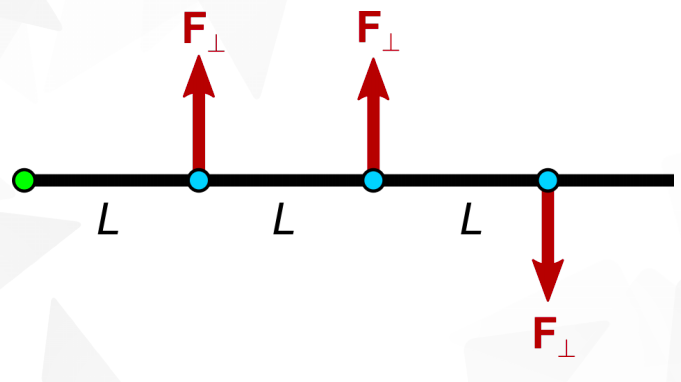
\includegraphics[scale = 0.3]{figs/D3/disc_a.png}}
      \subfigure[]{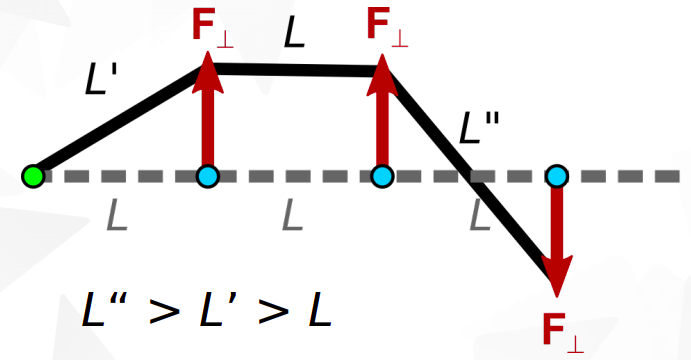
\includegraphics[scale = 0.3]{figs/D3/disc_b.png}}
      \subfigure[]{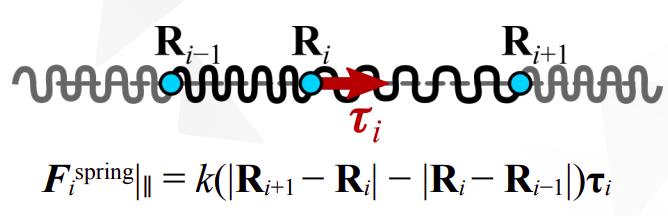
\includegraphics[scale = 0.35]{figs/D3/disc_c.png}}
      \caption{Al discretizar (a) las fuerzas pueden provocar que el camino entre imágenes no se conserve (b). Esto se soluciona utilizando resortes (c).}
      \label{fig:disc}
  \end{figure}

  Reuniendo toda la info rmación nos queda entonces que NEB consiste en (Fig. \ref{fig:NEB_disc}):
    \begin{enumerate}
      \item Conectar dos mínimos con un camino de reacción. Esto debe proponerse, pudiendo ser simplemente una interpolación lineal (default).
      \item Discretizar el camino de reacción mediante imágenes ($\left\{ \vec{R}_j \right\}_{j=1}^M$).
      \item Conectar las imágenes con resortes.
      \item Minimizar el camino de reacción mediante NEB: sobre la $j$-ésima imagen se aplica una fuerza perpendicular a la banda, moviéndola, y una tangencial que es la del resorte. Estos son los \emph{empujones} (nudgings) que dan lugar al nomnbre.
    \end{enumerate}

  \begin{figure}[H]
      \centering
      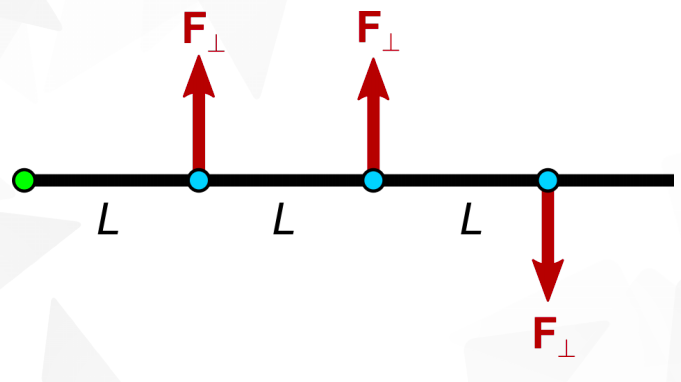
\includegraphics[scale = 0.4]{figs/D3/disc_a.png}
      \caption{NEB considerando discretización y resortes.}
      \label{fig:NEB_disc}
  \end{figure}

  La elección de la tangente es crucial para la convergencia. Una buena elección es considerar una tangente local, la cual sólo considera la imagen adyacente de mayor energía. En caso de que la imagen tenga menor energía que ambas imágenes adyacentes se toma un promedio.

  Como el interés está centrado en conocer el saddle, debemos aumentar la resolución de la zona. Para ello podemos usar constantes del resorte variables entre dos valores dados. Cuanto mayor sea la energía de la imagen, más rígido debe ser el resorte. Así la densidad de imágenes en la proximidad del saddle será mayor.

  En QE se pueden utilizar imágenes intermedias que permiten dar una guía para el camino de reacción inicial (Fig. \ref{fig:inter}). Muy útil cuando se tiene una intuición de la situación. Sólo son una guía, pero no se toman como imágnees para el cálculo.

  \begin{figure}[H]
      \centering
      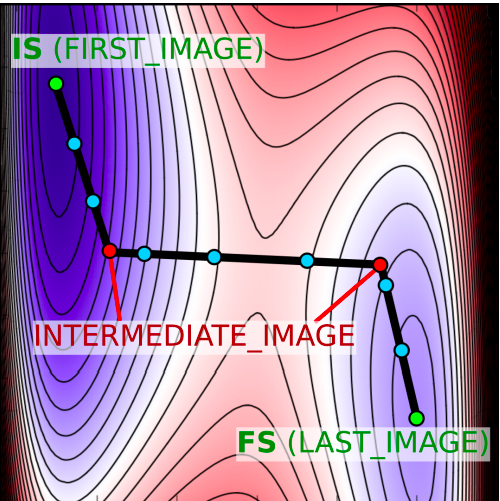
\includegraphics[scale = 0.4]{figs/D3/inter.png}
      \caption{Uso de imágenes intermedias.}
      \label{fig:inter}
  \end{figure}

\subsubsection{CI-NEB}

  Incluso cuando se tienen muchas imágenes y constantes de resorte variables, puede ocurrir que ninguna imagen quede lo suficientemente cerca del estado del saddle. Una solución al problema es recurrir al Climbing Image NEB (CI-NEB), donde se le permite a la imagen de mayor energía \emph{escalar} al desacoplarle los resortes. Para escalar necesitamos invertir la fuerza tangcial sobre la banda.

  \begin{figure}[H]
      \centering
      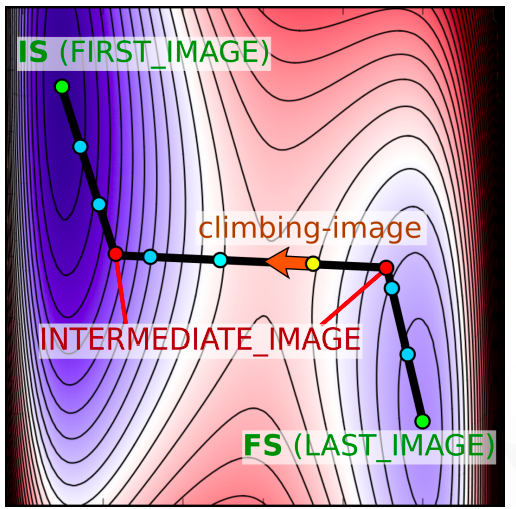
\includegraphics[scale = 0.4]{figs/D3/climb.png}
      \caption{Uso de imágenes intermedias en CI-NEB.}
      \label{fig:climb}
  \end{figure}

\subsection{neb.x}

  Se tienen dos bloques en el input: el primero contiene las especificaciones para NEB, mientras que en el segundo están las especificaciones para pw.x. En la parte del NEB tenemos una sección obligatoria donde definimos el camino de reacción y una parte opcional si queremos hacer CI-NEB (Figs. \ref{fig:nebx} y \ref{fig:nebx_2}). En la parte del PW tenemos que poner más cosas en la carta de posiciones (Fig. \ref{fig:pwx}).

  \begin{figure}[H]
      \centering
      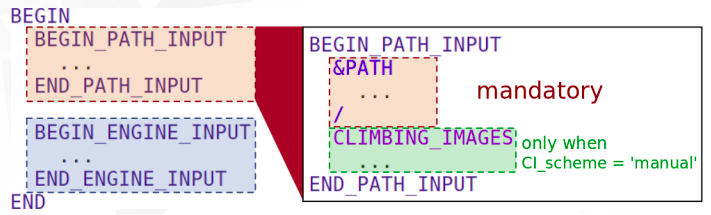
\includegraphics[scale = 0.4]{figs/D3/nebx.png}
      \caption{Input file: neb part.}
      \label{fig:nebx}
  \end{figure}

  \begin{figure}[H]
      \centering
      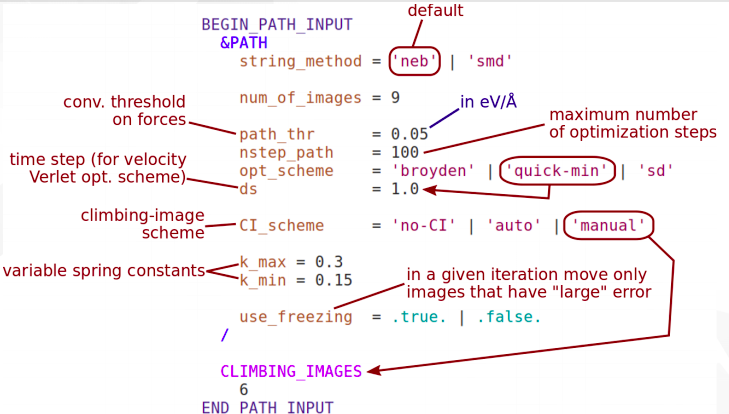
\includegraphics[scale = 0.4]{figs/D3/nebx_2.png}
      \caption{Input file: neb part con más detalles.}
      \label{fig:nebx_2}
  \end{figure}

  \begin{figure}[H]
      \centering
      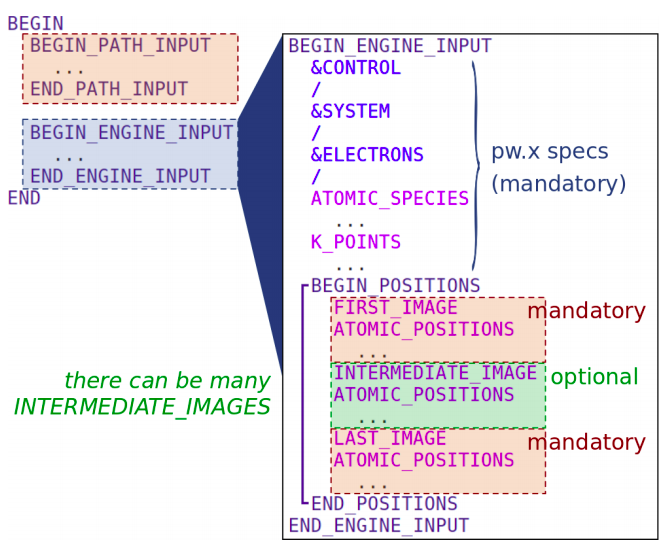
\includegraphics[scale = 0.4]{figs/D3/pwx.png}
      \caption{Input file: pw part.}
      \label{fig:pwx}
  \end{figure}

  Si usamos $use\_freezing = .true.$ el cálculo primero movera aquellas imágenes que tengan mayor error según algún criterio. Esto es conveniente: es mejor primero optimizar sólo aquellas imágenes de mayor error respecto al mínimo de energía (Fig. \ref{fig:nebxout}).

  \begin{figure}[H]
      \centering
      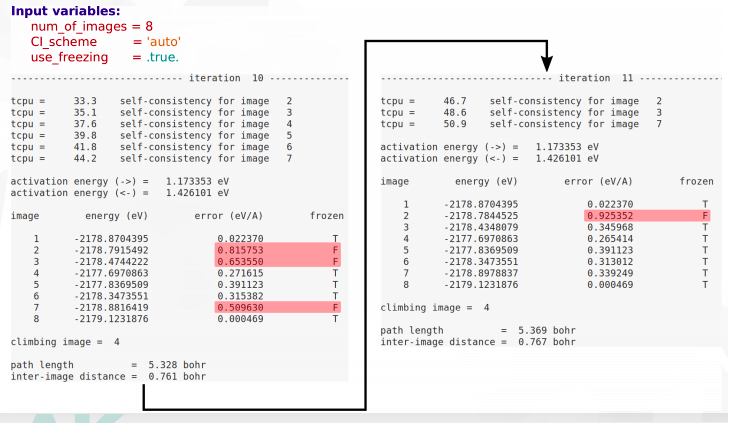
\includegraphics[scale = 0.5]{figs/D3/nebxout.png}
      \caption{Output file.}
      \label{fig:nebxout}
  \end{figure}

\subsection{Aspectos generales de NEB}

  Los cálculos NEB suelen tener una convergencia difícil. Por lo tanto es conveniente:
    \begin{itemize}
      \item Usar la experiencia es relevante: usar intuición química.
      \item Usar estados inicial y final ya relajados. En este sentido, no conviene utilizar $first\_last\_opt = .true.$.
      \item Usar imaǵenes intermedias.
    \end{itemize}

  La cantidad de imágenes a utilizar es variable. Una distancia entre imágenes de 1 ó 2 Bohr suele ser suficiente. Esta distancia se imprime en el output por lo que se recomiendo hacer un dryrun haciendo $nstep_path = 0$ (Fig. \ref{fig:dryrun}).

  \begin{figure}[H]
      \centering
      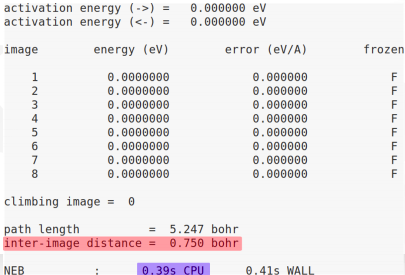
\includegraphics[scale = 0.7]{figs/D3/dryrun.png}
      \caption{Dryrun para conocer la distancia entre imágenes.}
      \label{fig:dryrun}
  \end{figure}

  Es bueno visualizar previamente el camino de reacción inicial antes de hacer el cálculo. Esto se puede hacer con xcrysden:
    $$xcrysden \quad --pwi \quad neb.in$$

  Es conveniente calcular un paso elemental a la vez (una única saddle). La opción $CI\_scheme = 'manual'$ permite calcular varios saddle en simultáneo.

  Usar $use\_freezing = .true.$ suele ser beneficioso.

  Respecto a los valores de las constantes de resorte mínima y máxima, no son tan importantes para el cálculo: el default suele funcionar bien. De lo contrario, en el output el programa sugiere valores.

  No es conveniente activar CI-NEB desde el comienzo. Primero debemos relajar el camino de reacción para lograr la mayor estabilidad posible. Recién ahí activamos el CI-NEB ($CI\_scheme = 'auto'$). Esto es porque a medida que avanzan las iteraciones puede ir cambiando qué imagen es la de mayor energía, dando lugar a oscilaciones. Esto se puede setear e PWTK (Fig. ).

  \begin{figure}[H]
      \centering
      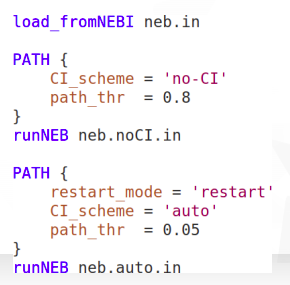
\includegraphics[scale = 0.8]{figs/D3/PWTK.png}
      \caption{Cómo escribir en PWTK para tener CI-NEB apagado al comienzo y luego encenderlo.}
      \label{fig:PWTK}
  \end{figure}

  No deben intercambiarse las posiciones (los índices) de los átomos en el input: las inconsistencias se rompe el programa.

  You cannot do:
  xcrysden --pwo neb.out
  Why? Look into the neb.out output file and you will notice there are no atomic coordinates there.
  Instead, neb.x writes a number of prefix.* files, in particular:
  prefix.dat -- energies of images
  prefix.int -- interpolated energies on a denser grid (larger number of images)
  prefix.axsf -- xcrysden XSF file for visualization
  etc.
  Hence you can do: xcrysden --xsf prefix.axsf
  Where prefix is as set in the input (e.g. H2+H, ...). Do "ls" and you will notice these files.

\section{Q\&A 2/2}

\definicion{I have heard that doing a CI-NEB calculation is not enough to assert that the saddle point found is the transition state. In addition to that, a phonon calculation must be done. The obtained state can be considered as the transition state only if we obtain imaginary frequencies. Is that true ?}

In general yes, however the CI-NEB should get you close enough for all practical purposes, at least for systems that you can't afford a phonon calculation

\definicion{How chemisorbtion is different from physiorbtion in qe and how they are performed}

Short answer: QE doesn't care, it calculates from first principles.
Note however that dispersion interactions are not described by plain DFT functionals, hence you need to use some special functional or a semi-empiric dispersion correction: you will learn that tomorrow.

\definicion{In order to have the best IS and FS in neb calculations can we perform a preliminar 'relax' or 'vc-relax' calculations of both the IS and the FS and then use the structural optimized parameters to perform the neb calculation? Or there are other ways to do that?}

Yes, this is my recommendation, i.e. optimize the first and the last image, then make intermediate images (if needed) and only then do NEB calc.
I am not sure vc-relax NEB is implemented in QE (I have never used it)

\definicion{we have to keep the same lattice parameters in both IS and FS? right?}

Yes. In the input on neb, you have to enter the common lattice parameter.

\section{Hands-on}

\definicion{Topic:} Optimizations, NEB. Automating the workflow (PWTK).

\definicion{Speaker:} Ari Paavo SEITSONEN (École Normale Supérieure, Paris).

\subsection{relax}

\subsubsection{Objetivo}

  Realizar una optimización estructural de las posiciones atómicas, tanto con grafeno como con óxido de grafeno.

\subsubsection{Pasos}

  Para el caso del grafano (grafeno con un H en cada C en trans):

    \begin{enumerate}
      \item Notar que en el input ahora hay una nueva namelist: \&IONS. Correr con
        \begin{verbatim}
          pw.x -in pw.graphane.relax.in > pw.graphane.relax.out &
        \end{verbatim}
      \item Analizar el output: son sucesivos pasos de SCF seguidos de cálculos de fuerzas para determinar las nuevas posiciones atómicas.
      \item visualizar la evolución estructural.
        \begin{verbatim}
          xcrysden --pwo pw.graphane.relax.out
        \end{verbatim}
    \end{enumerate}

  Para el óxido de grafeno (átomo de grafeno adsorbido sobre una celda 3x3 de grafeno) hacer lo mismo: hacer la relajación y luego visualizarla.

    \begin{verbatim}
      pw.x -in pw.graphene3x3-O.relax.in > pw.graphene3x3-O.relax.out &
      xcrysden --pwo pw.graphane.relax.out
    \end{verbatim}

\subsubsection{Resultados: relax}

  Primero analizamos el grafano. En 5 ciclos SCF converge:

    !    total energy              =     -24.78069777 Ry
         estimated scf accuracy    <          1.4E-09 Ry
    !    total energy              =     -25.01952054 Ry
         estimated scf accuracy    <          2.0E-09 Ry
    !    total energy              =     -25.10918098 Ry
         estimated scf accuracy    <          6.3E-09 Ry
    !    total energy              =     -25.11219615 Ry
         estimated scf accuracy    <          1.2E-09 Ry
    !    total energy              =     -25.11408866 Ry
         estimated scf accuracy    <          9.5E-11 Ry
    !    total energy              =     -25.11411542 Ry
         estimated scf accuracy    <          2.6E-10 Ry

  A partir de la figura vemos que se acomoda en su disposición tetraédrica dada la hibridización sp3. Se peude ver que la saturación provoca que pierda parte de sus propiedades eléctricas. Por eso todo lo respecto al smearing está comentado en el input.

  \begin{figure}[H]
      \centering
       \subfigure[]{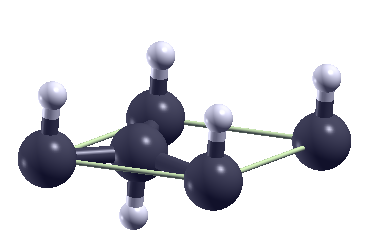
\includegraphics[scale = 0.30]{figs/D3/Grafano_in.png}}
       \subfigure[]{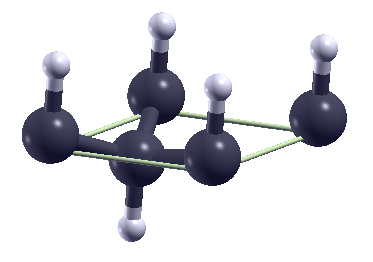
\includegraphics[scale = 0.30]{figs/D3/Grafano_out.png}}
       \caption{Grafano antes (a) y después (b) de la relajación.}
   \end{figure}

  Después tenemos un expoxi- sobre una superficie de grafeno en una cupercelda (es 3x3 pero también debería estudairse este tamaño medainte test de convergencia). En este caso sí usamos ocupación fraccionaria (smearing). Debería usarse una $k$-mesh de 3x3x3, pero se usó gamma para que sea más rápido. La distancia entre átomos de carbono es mayor para los que participan del epóxido respecto a los demás carbonos del grafeno. Esto se puede asociar a hibridización de cada uno de los C.

  \begin{figure}[H]
      \centering
       \subfigure[]{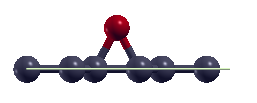
\includegraphics[scale = 0.30]{figs/D3/GrO_relax_in.png}}
       \subfigure[]{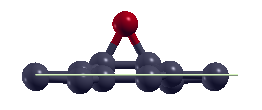
\includegraphics[scale = 0.30]{figs/D3/GrO_relax_out.png}}
       \caption{Grafeno oxidado con un grupo epoxi antes (a) y después (b) de la relajación.}
   \end{figure}

  \Obs{Como tenemos 2 átomos diferentes, deberíamos haber chequeado la convergencia de los cutoffs para ambos elementos y tomar el valor más alto.}

\subsection{vc-relax}

\subsubsection{Objetivo}

  Realizar un cálculo de optimización estructural, relajando también los parámetros de red.

\subsubsection{Pasos}

  Primero se analiza Zn bulk:
    \begin{enumerate}
      \item Analizar los cambios en el input y correr
        \begin{verbatim}
          pw.x -in pw.Zn.vc-relax.in > pw.Zn.vc-relax.out &
        \end{verbatim}
      \item Analizar el output: ciclos SCF, fuerzas y tensores de estrés llevan a nuevos parámetros de red y posiciones atómicas.
      \item Visualizar.
      \begin{verbatim}
        xcrysden --pwo pw.Zn.vc-relax.out
      \end{verbatim}
    \end{enumerate}

  Una alternativa es hacer un barrido bidimensional de ambos parámetros de red con
    \begin{verbatim}
      pwtk Zn-scan.pwtk
    \end{verbatim}

  La PES resultante se puede ver con
    \begin{verbatim}
      gnuplot plot2D.gp
    \end{verbatim}

  Luego se analiza un cristal molecular de urea:
    \begin{enumerate}
      \item Ejecutar
      \begin{verbatim}
        pw.x -in pw.urea.vc-relax.in > pw.urea.vc-relax.out &
      \end{verbatim}
    \end{enumerate}

  \Obs{Estos cálculos ya son bastante más pesados así que conviene mandarlos al cluster.}

\subsubsection{Resultados: vc-relax}

  Empezamos con el cluster de Zn. Primero hacemos una relajación con un par de CI fijas: el programa buscará el mínimo. Vemos que la celda se agranda:
    $$celldm(1) =  4.8 \Rightarrow celldm(1) = 4.96 \Rightarrow a = 2.62\ \si{\angstrom}$$
    $$celldm(3) =  1.8 \Rightarrow celldm(3) = 2.02 \Rightarrow c = 5.29\ \si{\angstrom}$$

  \begin{figure}[H]
      \centering
       \subfigure[]{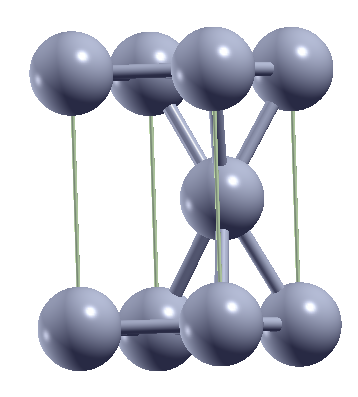
\includegraphics[scale = 0.30]{figs/D3/Zn_vc_in.png}}
       \subfigure[]{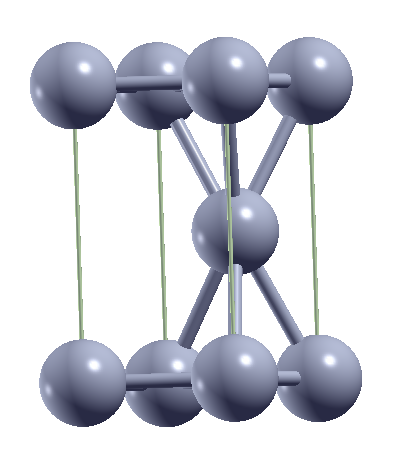
\includegraphics[scale = 0.30]{figs/D3/Zn_vc_out.png}}
       \caption{Bulk de Zn antes (a) y después (b) de la relajación tanto de posiciones atómicas como de parámetros de red.}
   \end{figure}

  \Obs{El orden de qué tan fácil es alcanzar la convergencia es: energías, fuerzas y estrés. A medida que avanzamos en dificultad, necesitamos cutoffs más altos.}

  La segunda opción es hacer un barrido bidimensional. En este caso no hacemos una vc-relax, sino que por cada par de CI hacemos una SCF. Aunque esto no da un valor tan exacto como el vc-relax, permite conocer la región donde se encuentra el mínimo. Luego puedo hacer una interpolación para hallar el mínimo o hacer un vc-relax pero dando CI cercanas al mínimo.

  Si vemos el mapa, podemos reconocer que el mínimo está aproximadamente en $a = 2.6\ \si{\angstrom}$ y $c = 5.2\ \si{\angstrom}$. Esto está bastante cerca de los valores calculados mediante vc-relax.

  \begin{figure}[H]
      \centering
       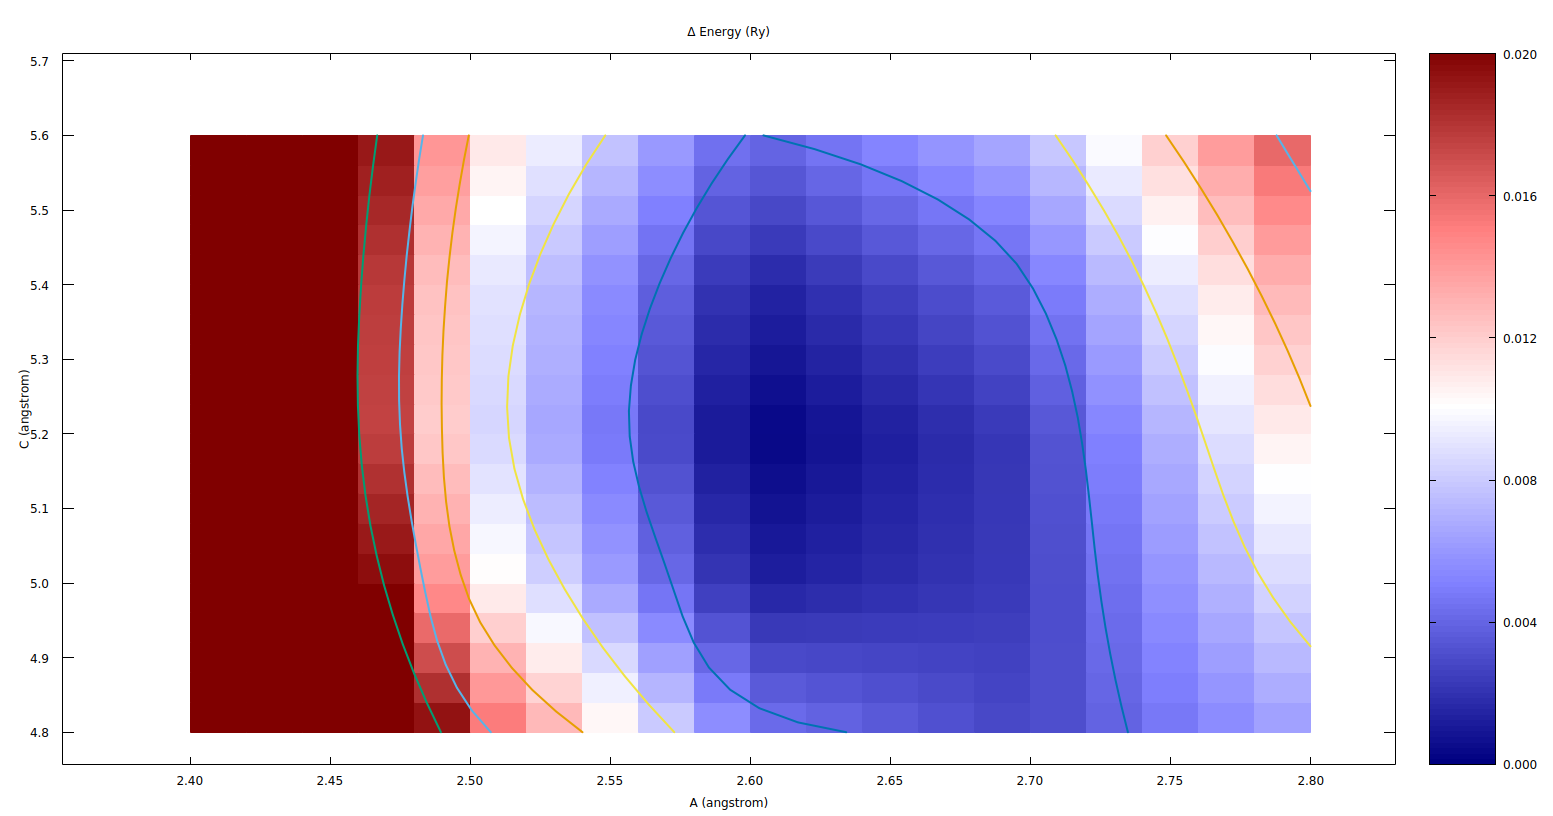
\includegraphics[scale = 0.30]{figs/D3/Zn_scan.png}
       \caption{Análisis bidimensional de los parámetros de red para el Zn bulk.}
   \end{figure}

  \Obs{En general ocurre que los parámetros de red calculados no coinciden completamente con los experimentales incluso habiendo elegido los valores que minimizan los errores, \emph{i.e.} habiendo estudiado la convergencia. Esto se debe al término de XC. Conviene usar los valores de nuestra convergencia para hacer los estudios: así los cálculos posteriores tendrán minimizadas sus fuentes de error.}

  En el caso de la urea tamibién se ve que la celda se agranda, pero el cambio es más sutil.

  \begin{figure}[H]
      \centering
       \subfigure[]{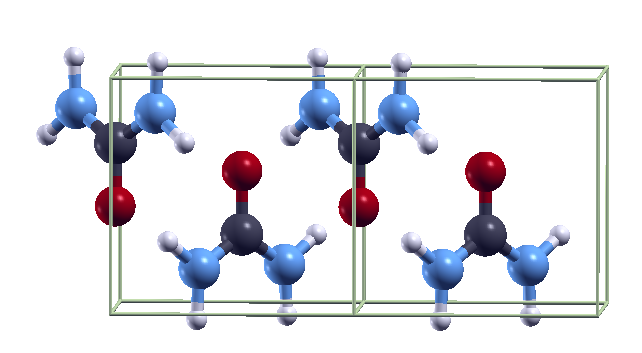
\includegraphics[scale = 0.30]{figs/D3/urea_vc_in.png}}
       \subfigure[]{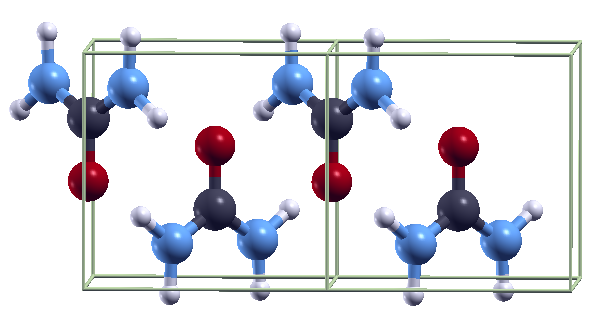
\includegraphics[scale = 0.30]{figs/D3/urea_vc_out.png}}
       \caption{Urea antes (a) y después (b) de la relajación tanto de posiciones atómicas como de parámetros de red.}
   \end{figure}

\subsection{NEB: transferencia de H}

\subsubsection{Objetivo}

  Hacer una búsqueda del estado de transición para una reacción química simple utilizando el método NEB (neb.x).

\subsubsection{Pasos}

  En el primero ejemplo tenemos una transferencia de protones: H + H2 --> H2 + H. Primero no utilizamos una imagen intermedia:

    \begin{enumerate}
      \item Solo se dan las imágenes inicial y final y neb.x hace una interpolación lineal con la cantida de imágenes deseadas. El camino de reacción inicial se puede visualziar con
        \begin{verbatim}
          xcrysden --pwi neb.H2+H.in
        \end{verbatim}
      \item Correr el programa.
      \begin{verbatim}
        neb.x -in neb.H2+H.in > neb.H2+H.out
      \end{verbatim}
      \item Analizar el output. ¿Cuántos pasos fueron necesarios para la convergencias? ¿Cuánto vale la barrera de activación?
      \item Plotear el MEP.
      \begin{verbatim}
        gnuplot H2+H.gp
      \end{verbatim}
      \item Visualizar las estructuras del MEP con alguno de los siguientes comandos.
      \begin{verbatim}
        xcrysden --xyz H2+H.xyz
        xcrysden --axsf H2+H.axsf
      \end{verbatim}
    \end{enumerate}

  Luego usamos una imagen intermedia:
    \begin{enumerate}
      \item Visualizar el camino inicial. Comparar con el caso anterior.
        \begin{verbatim}
          xcrysden --pwi neb.H2+H.w-inter-image.in
        \end{verbatim}
      \item Correr el programa.
      \begin{verbatim}
        neb.x -in neb.H2+H.w-inter-image.in > neb.H2+H.w-inter-image.out &
      \end{verbatim}
      \item Analizar el output. Comparar barreras de activación
    \end{enumerate}

    \begin{figure}[H]
        \centering
          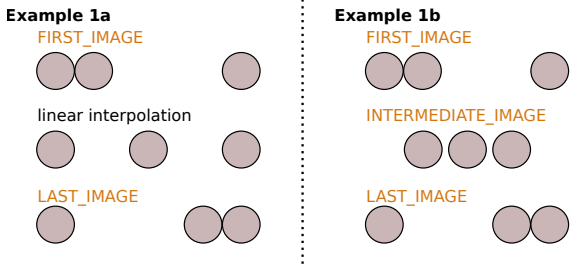
\includegraphics[scale = 0.6]{figs/D3/imagen_intermedia.png}
         \caption{Comparación entre no usar (a) y usar (b) imagen intermedia.}
     \end{figure}

\subsubsection{Resultados: transferencia de H}

  La reacción es una transferencia de protones. En el primer ejemplo no utilizamos imágnes intermedias: sólo especificamos la primera imágen (reactivos) y la última (productos). El camino de reacción se discretiza en 7 imágenes y neb.x hace una interpolación lineal para ubicar las faltantes. El segundo ejemplo aprovecha un poco de intuición química para intentar dar un mejor camino de reacción inicial. Dada la ayuda que le damos al programa, la convergencia se alcanzará en menos pasos.

  \Obs{El umbral de convergencia $path\_thr = 0.1$ no es el óptimo, sino que se eligió para que corriera más rápido.}

  \begin{figure}[H]
      \centering
       \subfigure[]{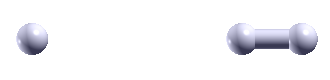
\includegraphics[scale = 0.30]{figs/D3/NEB_H3_noint_in.png}}
       \subfigure[]{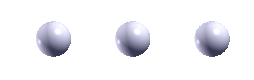
\includegraphics[scale = 0.30]{figs/D3/NEB_H3_int.png}}
       \subfigure[]{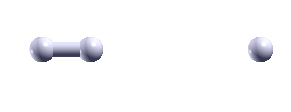
\includegraphics[scale = 0.30]{figs/D3/NEB_H3_noint_out.png}}
       \caption{Transferencia de protones: punto inicial (a) y final (c) de la reacción. En (b) se tiene la imagen intermedia considerada.}
   \end{figure}

  La corrida con imagen intermedia terminó en unos 5 minutos, mientras que la otra ya va más de 45 minutos. Sus perfiles son iguales: la simetría es porque en reactivos y productos tenemos exactamente lo mismo. Sin embargo, se ve que la corrida sin imagen itnermedia alcanza una barrera de activación mayor: sin imagen itnermedia se llega a 0.2844 eV, mientras que con imagen intermedia tenemos 0.2690 eV. De todas formas la diferencia no es significativa, poniendo en relevancia que es mejor hacer el cálculo con imagen intermedia.

  \begin{figure}[H]
      \centering
       \subfigure[]{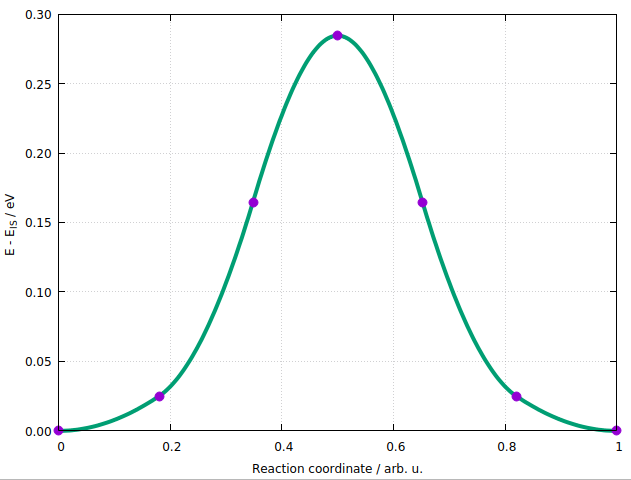
\includegraphics[scale = 0.45]{figs/D3/NEB_H3_L.png}}
       \subfigure[]{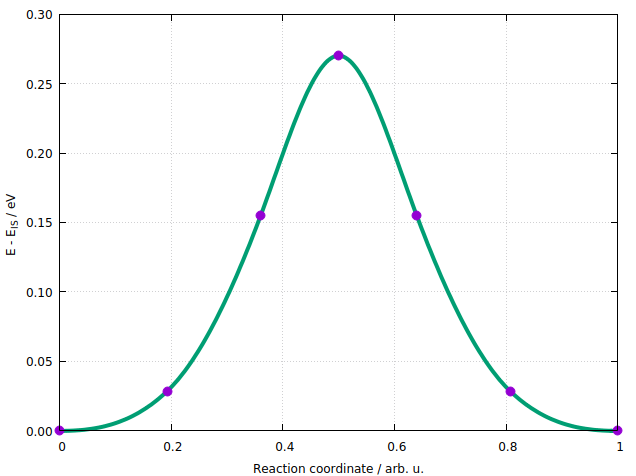
\includegraphics[scale = 0.45]{figs/D3/NEB_H3_C.png}}
       \caption{Perfil de reacción sin (a) y con (b) iamgen intermedia.}
   \end{figure}

\subsection{NEB: disociación de H}

\subsubsection{Objetivo}

   Llevar a cabo una NEB no trivial.

\subsubsection{Pasos}

  No sólo usaremos imágenes intermedias, sino que además dividiremos el cálculo NEB en dos etapas para así ayudar a la convergencia ya que haremos CI-NEB: primero haremos una NEB común ($CI\_scheme = 'no-CI'$) para estabilizar un poco el camino de reacción y, luego, permitimos que escale ($CI\_scheme = 'auto'$). Esto es más fácil de hacer usando PWTK. En la primera etapa el umbral de convergencia es mayor.

       \begin{enumerate}
         \item Visualizar el camino de reacción inicial.
           \begin{verbatim}
             xcrysden --pwi neb.H2-diss.Al100-2x1-2L.in
           \end{verbatim}
          \item Correr el programa.
          \begin{verbatim}
            remote_pwtk neb.pwtk
          \end{verbatim}
          \item Cuando termina, traer los resultados.
          \begin{verbatim}
            rsync_from_hpc '*.out'
          \end{verbatim}
          \item Analizar resultados. ¿Cuántos pasos necesito la convergencia? ¿Cuál es la barrera de activación?
          \item Graficar el MEP.
          \begin{verbatim}
            gnuplot H2-diss.Al100-2x1-2L.gp
          \end{verbatim}
          \item Visualizar los cambios estructurales.
          \begin{verbatim}
            xcrysden --axsf H2-diss.Al100-2x1-2L.axsf
          \end{verbatim}
       \end{enumerate}

\subsubsection{Resultados: disociación de H}

  Tenemos la disociación de hidrógeno molecular sobre AL(100).

  \begin{figure}[H]
      \centering
       \subfigure[]{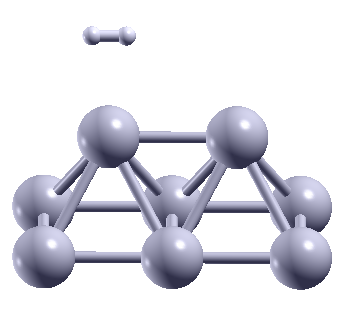
\includegraphics[scale = 0.30]{figs/D3/diss_ini.png}}
       \subfigure[]{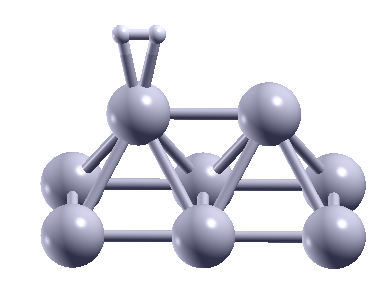
\includegraphics[scale = 0.30]{figs/D3/diss_inter.png}}
       \subfigure[]{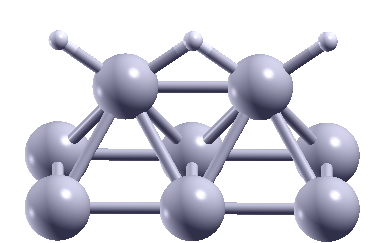
\includegraphics[scale = 0.30]{figs/D3/diss_fin.png}}
       \caption{Disociación de hidrógeno molecular sobre AL(100): punto inicial (a) y final (c) de la reacción. En (b) se tiene la imagen intermedia considerada.}
   \end{figure}

  Se puede ver que la barrera de activación es de 1.17 eV. La asimetría de la curva es porque los productos son más estables que los reactivos.

   \begin{figure}[H]
       \centering
        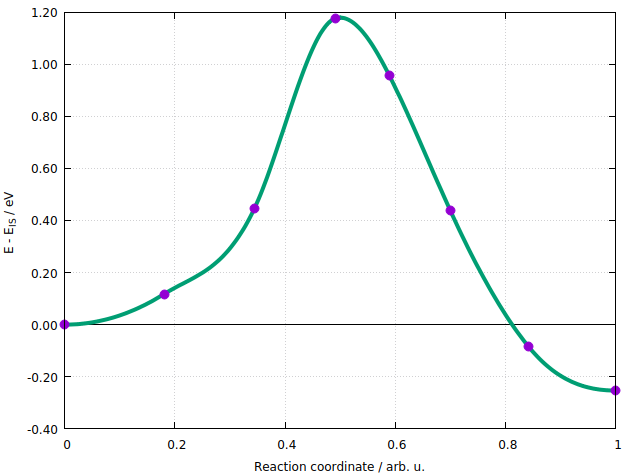
\includegraphics[scale = 0.45]{figs/D3/diss.png}
        \caption{Perfil de reacción para la disociación de hidrógeno molecular sobre AL(100).}
    \end{figure}

\subsection{pwtk automation}

\subsubsection{Objetivo}

  Se hacen diferentes pruebas con el fin de explorar las capacidades de PWTK.


This exercise consists from three examples, in particular:

* `ex1.eos/` -- how to use EOS utility of PWTK to calculate EOS of Rh bulk.

* `ex2.O@Al111/` -- how to run many calculations with a relatively
                    simple PWTK script; it calculates a 2D potential
                    energy surface of lateral positions of O @ Al(111).
                    It is also shown how one can automatically
                    tabulate calculated structures with PWTK.

* `ex3.CO@Rh100/` -- a more elaborate PWTK example that shows how to
                     glue together various calculations. In particular,
                     it analyzes the bonding of CO molecule on Rh(100).


**REMARK:** all three examples imports the `./common.pwtk` file, which
specifies the most common set of input data that is used by all
examples, i.e., list of pseudo-potentials, energy cutoffs,
smearing, ...


**BEWARE:** the cutoffs and convergence thresholds and other parameters are
very lousy as to speed-up calculations.


\subsubsection{Pasos}

  \begin{enumerate}
    \item
      \begin{verbatim}

      \end{verbatim}
  \end{enumerate}

\subsubsection{Resultados: pwtk automation}
